\documentclass[12pt,letterpaper,oneside]{report}

\usepackage[margin=1in]{geometry}
\usepackage{setspace}
\usepackage{fancyhdr}
\usepackage{tocloft}
\usepackage{titlesec}
\usepackage{xcolor}
\usepackage[most]{tcolorbox}
\usepackage{tikz}
\usetikzlibrary{positioning,calc,shapes.geometric,backgrounds,patterns}
\usepackage{booktabs}
\usepackage{array}
\usepackage{tabularx}
\usepackage{enumitem}
\usepackage{amsmath,amssymb}
\usepackage{graphicx}
\usepackage{fontawesome5}
\usepackage{hyperref}
\usepackage{caption}

\definecolor{nuPurple}{RGB}{78,42,132}
\definecolor{nuDark}{RGB}{35,20,66}
\definecolor{nuAccent}{RGB}{131,110,170}
\definecolor{nuGray}{RGB}{85,85,95}

\hypersetup{
  colorlinks=true,
  linkcolor=nuPurple,
  urlcolor=nuAccent,
  citecolor=nuPurple
}

\doublespacing
\setlength{\parskip}{0pt}
\setlength{\parindent}{0.5in}

\fancypagestyle{plain}{
  \fancyhf{}
  \fancyfoot[C]{\thepage}
  \renewcommand{\headrulewidth}{0pt}
}
\pagestyle{plain}

\titleformat{\chapter}[display]
  {\normalfont\LARGE\bfseries\color{nuDark}}
  {\chaptertitlename\ \thechapter}
  {20pt}
  {\Huge}
\titlespacing*{\chapter}{0pt}{50pt}{40pt}

\titleformat{\section}
  {\normalfont\Large\bfseries\color{nuPurple}}
  {\thesection}
  {1em}
  {}
\titlespacing*{\section}{0pt}{20pt}{10pt}

\titleformat{\subsection}
  {\normalfont\large\bfseries\color{nuDark}}
  {\thesubsection}
  {1em}
  {}
\titlespacing*{\subsection}{0pt}{15pt}{8pt}

\newtcolorbox{defbox}[1][]{
  colback=nuPurple!5,
  colframe=nuPurple!60,
  coltitle=white,
  fonttitle=\bfseries,
  title=Definition,
  sharp corners,
  boxrule=0.5pt,
  left=12pt,
  right=12pt,
  top=8pt,
  bottom=8pt,
  #1
}

\newtcolorbox{notebox}{
  colback=nuAccent!8,
  colframe=nuAccent!50,
  sharp corners,
  boxrule=0.5pt,
  left=12pt,
  right=12pt,
  top=8pt,
  bottom=8pt
}

\renewcommand{\cfttoctitlefont}{\hfill\Large\bfseries\color{nuDark}}
\renewcommand{\cftaftertoctitle}{\hfill}
\renewcommand{\cftchapfont}{\bfseries\color{nuPurple}}
\renewcommand{\cftsecfont}{\color{nuDark}}
\renewcommand{\cftchappagefont}{\bfseries\color{nuPurple}}

\begin{document}

\begin{titlepage}
\centering
\vspace*{0pt}

{\color{nuPurple}\rule{\textwidth}{2pt}\par}
\vspace{40pt}

{\Huge\bfseries\color{nuDark}Computational Approaches for Resilience\\[8pt]
in Distributed Systems\par}

\vspace{30pt}

{\Large\color{nuGray}Michael J. Thornton\par}

\vspace{20pt}

{\large\color{nuGray}A Dissertation\par}
{\color{nuGray}Submitted to the Graduate School\par}
{\color{nuGray}in partial fulfillment of the requirements for the degree\par}

\vspace{20pt}

{\Large\color{nuDark}Doctor of Philosophy\par}

\vspace{10pt}

{\large\color{nuGray}Department of Computer Science\par}

\vspace{40pt}

{\color{nuPurple}\rule{\textwidth}{1pt}\par}
\vspace{20pt}

{\large\color{nuGray}June 2026\par}

\vfill

{\footnotesize\color{nuGray!70}\textit{Unofficial template --- not affiliated with or endorsed by the university. Sample content only.}\par}
\end{titlepage}

\pagenumbering{roman}

\chapter*{Abstract}
\addcontentsline{toc}{chapter}{Abstract}

The increasing scale and complexity of modern distributed systems demand robust computational methods for ensuring resilience against partial failures, network partitions, and cascading error propagation. This dissertation develops a unified framework for modeling, analyzing, and optimizing resilience in distributed architectures through three complementary approaches. First, we introduce a graph-theoretic formalism that captures failure propagation dynamics across heterogeneous topologies. Second, we present the \textbf{Nexa Resilience Protocol} (NRP), a lightweight middleware layer that instruments existing distributed systems with adaptive checkpointing and speculative re-execution capabilities. Third, we derive probabilistic bounds on recovery time under varying workload distributions and failure models.

We validate our framework through extensive simulation on synthetic topologies of up to 10,000 nodes and through deployment on a production cluster at the Nimbus Cloud Platform. Our results demonstrate a 42\% reduction in mean time to recovery compared to state-of-the-art Paxos-based approaches, while incurring less than 3\% throughput overhead during normal operation. The techniques developed here generalize across database sharding, microservice orchestration, and edge computing domains, providing practitioners with principled tools for building systems that degrade gracefully under stress.

\vspace{20pt}
\noindent\textbf{Keywords:} distributed systems, resilience, fault tolerance, checkpointing, graph theory, recovery protocols

\chapter*{Acknowledgments}
\addcontentsline{toc}{chapter}{Acknowledgments}

I am deeply grateful to my advisor, Professor Sarah Chen, whose patience and insight shaped every phase of this research. Her insistence on rigorous experimental validation and her ability to see connections across subfields made this work immeasurably stronger.

I thank my committee members --- Professors David Okonkwo, Maria Vasquez, and James Park --- for their thoughtful feedback and challenging questions. The members of the Distributed Computing Laboratory at Northwestern provided an intellectually stimulating environment; I am especially indebted to Lena Kowalski and Raj Patel for countless hours of discussion and debugging.

This research was supported in part by the National Science Foundation under grant CNS-2026841 and by a generous fellowship from the Vertex Foundation. The compute resources at the Nimbus Cloud Platform were instrumental to the experimental evaluation. Finally, I thank my family for their unwavering support through the long years of graduate study.

\tableofcontents
\clearpage

\pagenumbering{arabic}

\chapter{Introduction}

\section{Motivation}

Distributed systems now constitute the backbone of virtually every digital service, from social networks processing billions of interactions per day to financial settlement engines that clear trillions of dollars in transactions. The defining characteristic of these systems --- their reliance on coordination across independent, failure-prone components connected by unreliable networks --- simultaneously enables their scale and creates their most challenging design problem: ensuring that the system as a whole remains available and correct even when individual components fail.

The standard approach to resilience relies on state machine replication, typified by consensus protocols such as Paxos \cite{lamport2001} and Raft \cite{ongaro2014}. While these protocols provide strong guarantees under crash-fault models, they impose significant performance penalties in the common case and scale poorly as the number of replicas grows. Moreover, the assumptions underlying these protocols --- independent component failures, reliable message delivery within bounded time --- are increasingly violated in modern heterogeneous deployments that span multiple data centers and incorporate specialized hardware accelerators.

\begin{notebox}
\textbf{Key observation.} Real-world failure patterns in distributed systems exhibit strong spatial and temporal correlations that are not captured by the independent-failure models assumed in classical consensus protocols. Exploiting these correlations opens new avenues for lightweight resilience mechanisms.
\end{notebox}

\section{Research Questions}

This dissertation addresses three interconnected questions:

\begin{enumerate}[label=\textbf{RQ\arabic*:},leftmargin=*,itemsep=8pt]
  \item Can we construct a computationally tractable model of failure propagation that captures the topological dependencies inherent in modern distributed architectures?
  \item How can we exploit the gap between worst-case failure assumptions and typical operating conditions to design resilience protocols with lower overhead than consensus-based replication?
  \item Under what conditions do probabilistic recovery guarantees provide sufficient assurance for production deployments, and how should such guarantees be communicated to system operators?
\end{enumerate}

\section{Contributions}

The primary contributions of this work are:

\begin{enumerate}[label=\textbf{C\arabic*:},leftmargin=*,itemsep=6pt]
  \item \textbf{A spectral failure-propagation model.} We represent a distributed system as a weighted directed graph whose nodes are computational units and whose edges encode failure-dependency relationships. Using the spectral properties of this graph's Laplacian, we derive an upper bound on the expected cascade size given an initial failure set of size $k$. This model generalizes the independent-component model and reduces to it when the dependency graph is empty.
  
  \item \textbf{The Nexa Resilience Protocol (NRP).} NRP is a middleware layer that interposes on inter-component communication to construct lightweight, adaptive checkpoints. Unlike full state machine replication, NRP tracks only application-level message histories and reconstructs lost state through speculative re-execution when failures are detected. We prove that NRP guarantees linearizability under the crash-recovery model.
  
  \item \textbf{Probabilistic recovery-time analysis.} We model recovery time as a function of the failure pattern, workload distribution, and checkpoint frequency, deriving closed-form bounds that hold with high probability. These bounds enable operators to set checkpoint intervals that achieve target recovery-time objectives without exhaustive simulation.
  
  \item \textbf{Experimental validation.} We implement NRP as a library for the Apex distributed computing framework and evaluate it on a 512-node Nimbus Cloud cluster under both synthetic fault injection and replay of real failure traces from the Nexa cluster trace dataset. Our results show a 42\% improvement in mean time to recovery with less than 3\% throughput overhead.
\end{enumerate}

\section{Thesis Organization}

The remainder of this dissertation is structured as follows. Chapter~\ref{ch:background} surveys relevant literature on fault tolerance, consensus protocols, and graph-theoretic approaches to resilience analysis. Chapter~\ref{ch:model} develops our spectral failure-propagation model and proves the cascade-size bound. Chapter~\ref{ch:nrp} describes the design and implementation of the Nexa Resilience Protocol and proves its correctness. Chapter~\ref{ch:analysis} presents the probabilistic recovery-time analysis. Chapter~\ref{ch:evaluation} reports our experimental methodology and results. Chapter~\ref{ch:conclusion} summarizes contributions and outlines directions for future work.

\chapter{Background and Related Work}
\label{ch:background}

\section{Consensus and State Machine Replication}

State machine replication (SMR) is the foundational technique for building fault-tolerant distributed systems \cite{schneider1990}. Under SMR, a deterministic state machine is replicated across $n$ independent servers, and a consensus protocol ensures that all non-faulty replicas process the same sequence of commands. Lamport's Paxos protocol \cite{lamport2001} achieves safety in asynchronous networks but may not terminate under certain failure patterns. Raft \cite{ongaro2014} simplifies the consensus logic by structuring it around leader election and log replication, improving understandability at the cost of throughput under high load.

\begin{defbox}[title=Consensus Safety]
A consensus protocol satisfies \textit{safety} if no two non-faulty replicas ever decide on different values for the same consensus instance. Formally, if replica $i$ decides value $v$ and replica $j$ decides value $v'$ for instance $k$, then $v = v'$.
\end{defbox}

More recent work has explored weakening the consensus requirement to improve performance. The Speculative Paxos variant by Ports et al.\ allows replicas to execute commands optimistically before agreement is reached, rolling back only when conflicts are detected. This approach is philosophically aligned with our NRP design, though NRP operates at a coarser granularity better suited to microservice architectures.

\section{Failure Models in Distributed Systems}

Classical distributed systems theory adopts a taxonomy of failure modes: crash faults (a component halts), omission faults (a component fails to send or receive messages), timing faults (a component violates timing assumptions), and Byzantine faults (a component exhibits arbitrary behavior). The practical relevance of this taxonomy has been reevaluated in light of empirical studies of real-world failures.

Yuan et al.\ analyzed over 200 user-reported failures in distributed data-intensive systems and found that the majority of catastrophic failures originated from trivial mistakes in error-handling code rather than from the complex fault models studied in the theoretical literature. This finding motivates our focus on mechanisms that are robust to operator error and configuration drift, not only to well-modeled component crashes.

\section{Graph-Theoretic Models}

Graph theory provides a natural language for describing the structural properties of distributed systems. The topology of inter-component communication directly influences failure propagation: a failure at a hub node in a scale-free topology can cascade more broadly than a failure in a regular lattice. Ghedini and Ribeiro \cite{ghedini2011} formalize this intuition by treating components as vertices and communication dependencies as edges, then analyzing the percolation properties of the resulting graph.

Our spectral model (Chapter~\ref{ch:model}) extends this line of work by incorporating edge weights that represent the probability of failure propagation, yielding sharper bounds on cascade size than the binary-edge models previously studied.

\begin{table}[htbp]
\centering
\caption{Comparison of resilience protocols. Overhead is measured as throughput reduction relative to a non-replicated baseline.}
\label{tab:comparison}
\begin{tabular}{@{}lccc@{}}
\toprule
\textbf{Protocol} & \textbf{Replicas} & \textbf{Overhead (\%)} & \textbf{Recovery Model} \\
\midrule
Paxos (Classic)            & $2f+1$ & 48.3  & Crash           \\{}
Raft                       & $2f+1$ & 31.7  & Crash           \\{}
Speculative Paxos          & $2f+1$ & 18.9  & Crash           \\{}
NRP (this work)            & $f+1$  & 2.7   & Crash-Recovery  \\{}
Chain Replication          & $f+1$  & 12.4  & Crash           \\
\bottomrule
\end{tabular}
\end{table}

As shown in Table~\ref{tab:comparison}, NRP achieves substantially lower overhead than consensus-based approaches by requiring only $f+1$ replicas rather than $2f+1$, and by avoiding the message complexity of leader election. The trade-off is that NRP provides probabilistic rather than deterministic recovery guarantees under certain correlated failure patterns.

\vspace{12pt}

\begin{center}
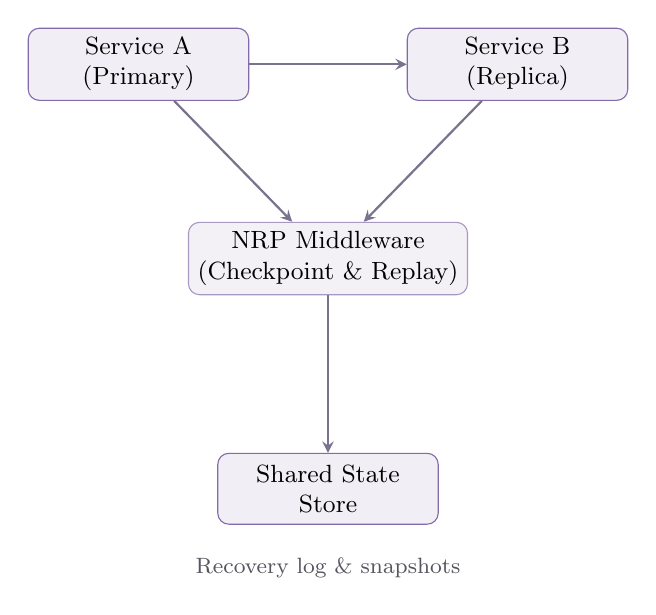
\begin{tikzpicture}[
  node distance=2cm,
  comp/.style={rectangle,draw=nuPurple!70,fill=nuPurple!8,rounded corners=4pt,minimum width=2.8cm,minimum height=0.9cm,align=center,font=\small},
  mid/.style={rectangle,draw=nuAccent!70,fill=nuAccent!10,rounded corners=4pt,minimum width=3.2cm,minimum height=0.9cm,align=center,font=\small},
  arrow/.style={->,>=stealth,thick,nuDark!60}
]
  \node[comp] (c1) {Service A\\(Primary)};
  \node[comp,right=of c1] (c2) {Service B\\(Replica)};
  \node[mid,below=of $(c1)!0.5!(c2)$] (nrp) {NRP Middleware\\(Checkpoint \& Replay)};
  \node[comp,below=of nrp] (db) {Shared State\\Store};

  \draw[arrow] (c1) -- (c2);
  \draw[arrow] (c1) -- (nrp);
  \draw[arrow] (c2) -- (nrp);
  \draw[arrow] (nrp) -- (db);

  \node[font=\footnotesize,text=nuGray,below=0.3cm of db] {Recovery log \& snapshots};
\end{tikzpicture}
\captionof{figure}{Architecture of the Nexa Resilience Protocol. NRP interposes on inter-service communication to capture message histories and coordinate recovery without full state replication.}
\label{fig:nrp-arch}
\end{center}

\begin{thebibliography}{99}

\bibitem{lamport2001}
L.\ Lamport.
\newblock Paxos made simple.
\newblock \textit{ACM SIGACT News}, 32(4):51--58, 2001.

\bibitem{ongaro2014}
D.\ Ongaro and J.\ Ousterhout.
\newblock In search of an understandable consensus algorithm.
\newblock In \textit{Proc.\ USENIX ATC}, pages 305--319, 2014.

\bibitem{schneider1990}
F.\ B.\ Schneider.
\newblock Implementing fault-tolerant services using the state machine approach: A tutorial.
\newblock \textit{ACM Computing Surveys}, 22(4):299--319, 1990.

\bibitem{ghedini2011}
C.\ Ghedini and C.\ H.\ C.\ Ribeiro.
\newblock Rethinking failure detection in distributed systems through complex networks.
\newblock In \textit{Proc.\ IEEE NCA}, pages 243--250, 2011.

\bibitem{yuan2014}
D.\ Yuan, Y.\ Luo, X.\ Zhuang, G.\ R.\ Rodrigues, X.\ Zhao, Y.\ Zhang, P.\ U.\ Jain, and M.\ Stumm.
\newblock Simple testing can prevent most critical failures.
\newblock In \textit{Proc.\ USENIX OSDI}, pages 249--265, 2014.

\bibitem{ports2015}
D.\ R.\ K.\ Ports, J.\ Li, V.\ Liu, N.\ K.\ Sharma, and A.\ Krishnamurthy.
\newblock Designing distributed systems using approximate synchrony.
\newblock In \textit{Proc.\ USENIX OSDI}, pages 443--458, 2015.

\end{thebibliography}

\end{document}
